% !TEX root = rampMeteringViaTheAdjoint.tex

\subsection{Junction model}\label{sub:junction-model}
We consider a junction $i$ with one incoming mainline $i$, modeled by the real interval $(-\infty, 0]$, with outgoing flux $f_i^{\text{out}}(t)$, one outgoing mainline $i+1$, modeled by the real interval $[0, +\infty)$, with incoming flux $f^{\text{in}}_{i+1}(t)$, one onramp, and one offramp. The density on the mainline satisfies the PDE
\[
\partial_t \rho_i(x, t) + \partial_x f(\rho_i(x, t)) = 0
\]
The onramp is modeled by a buffer, with size $l_i(t)$. The dynamics of the ramp buffer are simply given by the ODE
\begin{align}
\frac{d}{dt} l(t) &= \bar{D}_i(t) - r_i(t) \\
l_i(0) &= l_i^0
\end{align}
where $l_i^0$ is a given initial size for the buffer, and $r_i(t)$ is the outgoing flux from the ramp, given by solving the junction problem.
\begin{align*}
d_i(t) &= \begin{cases}
\min (u_i(t), r_i^{\max}) & \text{if } l_i(t) > 0 \\
\min (u_i(t), r_i^{\max}, \bar{D}_i(t)) & \text{if } l_i(t) = 0
\end{cases} \\
\delta_i(t) &= \min\left(F_i, v_i \rho_i(t) \right) \\
\sigma_{i+1}(t) &= \min \left( F_{i+1}, w_{i+1} \left( \rho_{i+1}^{\text{jam}} - \rho_{i+1}(t) \right) \right) \\
f_{i+1}^{\text{in}}(t) &= \min \left( (1-\beta_i)\delta_i(t) + d_i(t), \sigma_{i+1}(t)\right)
\end{align*}
finally, the outgoing flux from the mainline $f_i(t)$ and the outgoing flux from the ramp $r_i(t)$ are given by the solution to the following problem
\begin{equation}
\begin{aligned}
& \text{minimize} && \left\| \left(\begin{array}{c} r_i(t) \\ f_i^{\text{out}}(t) \end{array} \right) - \left(\begin{array}{c} r_i(t) \\ f_i^{\text{out}}(t) \end{array} \right) \cdot \alpha^{P_i} \alpha^{P_i} \right\|_2^2\\
& \text{subject to} && f_{i+1}^{\text{in}}(t) = (1-\beta_i)f_i^{\text{out}}(t) + r_i(t) \\
&&& r_i(t) \leq d_i(t) \\
&&& f_i^{out}(t) \leq \delta_i(t) \\
\end{aligned}
\end{equation}
where $\alpha^{P_i}$ is the normalized vector
\[
\alpha^{P_i} = \frac{1}{\sqrt{P_i^2 + (1-P_i)^2}} \left(\begin{array}{c} P_i \\ 1-P_i\end{array}\right)
\]
This junction model ensures that the flux into the mainline is maximized, and the flux solution of the junction solver is unique (the objective function of the optimization problem is a non-degenerate quadratic, thus strictly convex). The optimization problem guarantees a unique solution, by minimizing the distance to the line $\Delta_i^{P}: f_i^{\text{out}}(t) = \frac{P_i}{1-P_i} r_i(t)$.

\begin{figure}[h]
\centering
\subfloat[Intersection inside the feasible set]{
\resizebox{.5\columnwidth}{!}{
	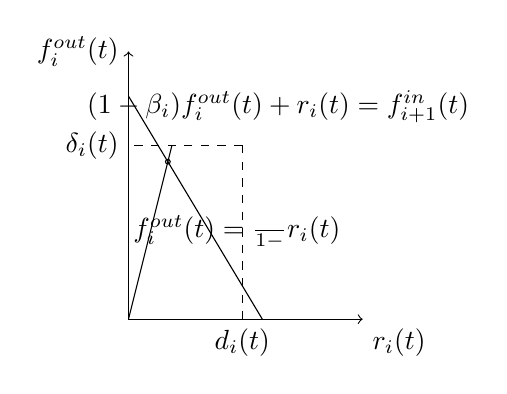
\begin{tikzpicture}[scale=1*.85,domain=0:1]

\def \rampDem{1.7}
\def \dem{2.6}
\def \priorityRat{0.8}
\def \splitRat{0.4}
\def \totalFlow{2}
\FontSmall


\coordinate (Z) at (0,0);
\coordinate (I1) at (\rampDem, 0);
\coordinate (I2) at (0, \dem);
\coordinate (I3) at (\rampDem, \dem);
\coordinate (A) at (0, {\totalFlow/(1-\splitRat)});
\coordinate (B) at (\totalFlow, 0);
\coordinate (C) at ({(1-\priorityRat)/\priorityRat*\dem}, \dem);

\draw[->] (Z) -- (3.5,0) node[below right]{$r_i(t)$};
\draw[->] (Z) -- (0,4) node[left]{$f^{\text{out}}_i(t)$};
\draw[dashed] (I3) -- (I1) node[below]{$d_i(t)$};
\draw[dashed] (I3) -- (I2) node[left]{$\delta_i(t)$};
\draw (A) -- (B) node[yshift=2.7cm, xshift=0.2cm]{$(1-\beta_i)f_i^{\text{out}}(t) + r_i(t) = f_{i+1}^{\text{in}}(t)$};
\draw (Z) -- (C) node[midway, xshift=1.1cm]{$f_i^{\text{out}}(t) = \frac{\priority{\icell}}{1-\priority{\icell}} r_i(t)$};
\draw (intersection of A--B and Z--C) circle (1pt);

\end{tikzpicture}
}
\label{fig:junctionFlowsInside}
}
\subfloat[Intersection outside the feasible set]{
\resizebox{.5\columnwidth}{!}{
	
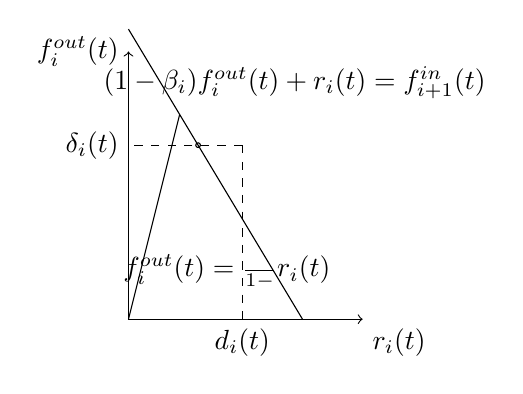
\begin{tikzpicture}[scale=1*.85,domain=0:1]

\def \rampDem{1.7}
\def \dem{2.6}
\def \priorityRat{0.8}
\def \splitRat{0.4}
\def \totalFlow{2.6}
\FontSmall

\coordinate (Z) at (0,0);
\coordinate (I1) at (\rampDem, 0);
\coordinate (I2) at (0, \dem);
\coordinate (I3) at (\rampDem, \dem);

\coordinate (A) at (0, {\totalFlow/(1-\splitRat)});
\coordinate (B) at (\totalFlow, 0);
\coordinate (C) at ({(1-\priorityRat)/\priorityRat*\dem}, \dem);
\coordinate (D) at (intersection of A--B and Z--C);


\draw[->] (Z) -- (3.5,0) node[below right]{$r_i(t)$};
\draw[->] (Z) -- (0,4) node[left]{$f^{\text{out}}_i(t)$};

\draw[dashed] (I3) -- (I1) node[below]{$d_i(t)$};
\draw[dashed] (I3) -- (I2) node[left]{$\delta_i(t)$};


\begin{scope}
%\clip (Z) rectangle (3.5,4);
\draw (A) -- (B) node[yshift=3cm, xshift=-0.1cm]{$(1-\beta_i)f_i^{\text{out}}(t) + r_i(t) = f_{i+1}^{\text{in}}(t)$};
\end{scope}

\draw (Z) -- (D) node[yshift=-2cm, xshift=0.6cm]{$f_i^{\text{out}}(t) = \frac{\priority{\icell}}{1-\priority{\icell}} r_i(t)$};
\draw (intersection of A--B and I3--I2) circle (1pt);

\end{tikzpicture}
}
\label{fig:junctionFlowsOutside}
}
\caption{Junction flows given by the junction solver}
\label{fig:junctionFlows}
\end{figure}

%-----------------------------------------------------------------------------------------------------------------------------------------------------------------
\subsection{Riemann problem}

We consider a Riemann problem at junction $i$ and at time $t_0$, where the inputs are constant in time, and we look for a flux solution that is also constant in time (until the next shock), thus we will drop the dependency on time in the input flux and the junction fluxes. Since the fluxes are constant, we have $\frac{d}{dt} l_i(t) = \bar{D}_i - r_i$, therefore the buffer size grows linearly in time.


TODO: define a solution to the Riemann problem

%-----------------------------------------------------------------------------------------------------------------------------------------------------------------
\subsection{Self-similar solution}

At $t_0^+$, starting from the solution $(\bar{\rho}_i(t_0), \bar{\rho}_{i+1}(t_0))$ of the Riemann solver, we show that the flux solution to the junction solver are invariant,
\[
\js_{l_i(t_0^+)}(\bar{\rho}_i(t_0), \bar{\rho}_{i+1}(t_0)) = \js{l_i(t_0)}(\rho_i(t_0), \rho_{i+1}(t_0))
\]
and as a consequence, the solution of the Riemann solver is invariant
\[
\rs_{l_i(t_0^+)} (\bar{\rho}_i(t_0), \bar{\rho}_{i+1}(t_0)) = (\bar{\rho_i}(t_0), \bar{\rho}_{i+1}(t_0))
\]
In other words, we need to show that $r_i(t_0^+) = r_i(t_0)$, and $f_i^{\text{out}}(t_0^+) = f_i^{\text{out}}(t_0)$.


%-----------------------------------------------------------------------------------------------------------------------------------------------------------------
\subsubsection{Initially empty buffer}
We first consider the case where the buffer is initially empty, $l_i(t_0) = 0$, and the input flux is greater than the output flux, i.e.  $\bar{D}_i > r_i$, and the buffer is growing linearly. Thus $l_i(t_0^+) > 0$. From these assumptions, the onramp demand is given by
\begin{align*}
d_i(t_0) &= \min (u_i, r_i^{\max}, \bar{D}_i) \\
d_i(t_0^+) &= \min (u_i, r_i^{\max})
\end{align*}

\paragraph{Remark} We observe that the ramp demand at time $t_0^+$ can only increase, i.e.
\begin{equation}
d_i(t_0^+) \geq d_i(t_0)
\label{eq:buffer-rampDemandIncrease}
\end{equation}
since
\begin{align*}
d_i(t_0^+)
&= \min (u_i, r_i^{\max})\\
&\geq \min (u_i, r_i^{\max}, \bar{D}_i) \\
& =d_i(t_0)
\end{align*}
Moreover, if $r_i(t_0) = d_i(t_0)$, then we have equality $d_i(t_0^+) = d_i(t_0)$. Proof: since $r_i(t_0) = d_i(t_0) = \min (u_i, r_i^{\max}, \bar{D}_i)$ and $r_i(t_0) < \bar{D}_i$ (the buffer is growing), we necessarily have $\min (u_i, r_i^{\max}) < \bar{D}_i$, thus $\min(u_i, r_i^{\max}) = \min (u_i, r_i^{\max}, \bar{D}_i)$.

%------------------------------------------------------------------------------
\paragraph{Supply-constrained case}
First, we assume that the junction is supply-constrained at time $t_0$, i.e. $(1-\beta_i)\delta_i(t_0) + d_i(t_0) > \sigma_{i+1}(t_0)$. Therefore the mainline supply at time $t_0^+$ is
\begin{equation}
\sigma_{i+1}(t_0^+) = \sigma_{i+1}(t_0)
\label{eq:buffer-supplyIncrease}
\end{equation}

We consider three cases, depending on the flux solution of the junction solver.

\begin{figure}[h]
\centering
\subfloat[Solution on the boundary $r_i = d_i$]{
\resizebox{.33\columnwidth}{!}{
	\def \scale{1.5}
\begin{tikzpicture}[scale=\scale,domain=0:1]

\def \rampDem{1.7}
\def \dem{2.2}
\def \demPlus{2.5}
\def \priorityRat{0.2}
\def \splitRat{0.4}
\def \totalFlow{2.2}

\coordinate (Z) at (0,0);
\coordinate (I1) at (\rampDem, 0);
\coordinate (I2) at (0, \dem);
\coordinate (I2') at (0, \demPlus);
\coordinate (I3) at (\rampDem, \dem);
\coordinate (I3') at (\rampDem, \demPlus);
\coordinate (A) at (0, {\totalFlow/(1-\splitRat)});
\coordinate (B) at (\totalFlow, 0);
\coordinate (C) at ({(1-\priorityRat)/\priorityRat*\dem}, \dem);
\coordinate (D) at (intersection of A--B and Z--C);


\draw[->] (Z) -- (3.5,0) node[below right]{$r_i$};
\draw[->] (Z) -- (0,4) node[left]{$f^{\text{out}}_i$};

\draw (I3') -- (I1) node[below]{$d_i(t_0) = d_i(t_0^+)$};
\draw (I3') -- (I2') node[left]{$\delta_i(t_0^+)$};
\draw (A) -- (B) node[yshift=1cm, xshift=0cm]{};
\draw (Z) -- (D) node[midway, xshift=1cm]{};
\draw (intersection of A--B and I3--I1) circle (1pt) node[above right]{$(r_i(t_0^+), f_i^{\text{out}}(t_0^+))$};

\end{tikzpicture}
}
\label{fig:junctionBuffer-SupplyConstrained-Boundary1}
}
\subfloat[Solution on the boundary $f_i^{\text{out}} = \delta_i$]{
\resizebox{.33\columnwidth}{!}{
	\def \scale{1.5}
\begin{tikzpicture}[scale=\scale,domain=0:1]

\def \rampDem{1.7}
\def \rampDemPlus{2.0}
\def \dem{2.2}
\def \priorityRat{0.9}
\def \splitRat{0.4}
\def \totalFlow{2.2}

\coordinate (Z) at (0,0);
\coordinate (I1) at (\rampDem, 0);
\coordinate (I1') at (\rampDemPlus, 0);
\coordinate (I2) at (0, \dem);
\coordinate (I3) at (\rampDem, \dem);
\coordinate (I3') at (\rampDemPlus, \dem);
\coordinate (A) at (0, {\totalFlow/(1-\splitRat)});
\coordinate (B) at (\totalFlow, 0);
\coordinate (C) at ({(1-\priorityRat)/\priorityRat*\dem}, \dem);
\coordinate (D) at (intersection of A--B and Z--C);


\draw[->] (Z) -- (3.5,0) node[below right]{$r_i$};
\draw[->] (Z) -- (0,4) node[left]{$f^{\text{out}}_i$};

\draw (I3') -- (I1') node[below right]{$d_i(t_0^+)$};
\draw (I3') -- (I2) node[above left]{$\delta_i(t_0)$} node[below left]{$\delta_i(t_0^+)$};
\draw (A) -- (B) node[yshift=1cm, xshift=0cm]{};
\draw (Z) -- (D) node[midway, xshift=1cm]{};
\draw (intersection of A--B and I3--I2) circle (1pt) node[above right]{$(r_i(t_0^+), f_i^{\text{out}}(t_0^+))$};

\end{tikzpicture}
}
\label{fig:junctionBuffer-SupplyConstrained-Boundary2}
}
\subfloat[Solution in the interior of the feasible set]{
\resizebox{.33\columnwidth}{!}{
	% !TEX root = ../rampMeteringViaTheAdjoint.tex
\def \scale{1.5}
\begin{tikzpicture}[scale=\scale,domain=0:1]

\def \rampDem{1.7}
\def \rampDemPlus{2.0}
\def \dem{2.2}
\def \demPlus{2.5}
\def \priorityRat{0.6}
\def \splitRat{0.4}
\def \totalFlow{2.2}

\coordinate (Z) at (0,0);
\coordinate (I1) at (\rampDem, 0);
\coordinate (I1') at (\rampDemPlus, 0);
\coordinate (I2) at (0, \dem);
\coordinate (I2') at (0, \demPlus);
\coordinate (I3) at (\rampDem, \dem);
\coordinate (I3') at (\rampDemPlus, \demPlus);
\coordinate (A) at (0, {\totalFlow/(1-\splitRat)});
\coordinate (B) at (\totalFlow, 0);
\coordinate (C) at ({(1-\priorityRat)/\priorityRat*\dem}, \dem);
\coordinate (D) at (intersection of I2'--I3' and Z--C);


\draw[->] (Z) -- (3.5,0) node[below right]{$r_i$};
\draw[->] (Z) -- (0,4) node[left]{$f^{\text{out}}_i$};

\draw[dashed] (I3) -- (I1) node[below left]{$d_i(t_0)$};
\draw[dashed] (I3) -- (I2) node[left]{$\delta_i(t_0)$};
\draw (I3') -- (I1') node[below right]{$d_i(t_0^+)$};
\draw (I3') -- (I2') node[left]{$\delta_i(t_0^+)$};

\draw (A) -- (B) node[yshift=1cm, xshift=0cm]{};
\draw (Z) -- (D) node[midway, xshift=1cm]{};
\draw (intersection of A--B and Z--D) circle (1pt) node[below]{$(r_i(t_0^+), f_i^{\text{out}}(t_0^+))$};

\end{tikzpicture}
}
\label{fig:junctionBuffer-SupplyConstrained-Interior}
}
\caption{Self-similar solution in the case of a supply-constrained junction problem at time $t_0$}
\label{fig:junctionBuffer-SupplyConstrained}
\end{figure}


%------------------------------------------------------------------------------
\paragraph{(a)} The intersection is on the boundary of the feasible set
\[
r_i(t_0) = d_i(t_0)
\]
By the previous remark, we have
\begin{align*}
d_i(t_0) = d_i(t_0^+)
\end{align*}
The mainline demand can only increase $\delta_i(t_0^+) \geq \delta_i(t_0)$ (in fact $\delta_i(t_0^+) = f_i^{\max}$), and by~\eqref{eq:buffer-supplyIncrease}, $\sigma_{i+1}(t_0^+) = \sigma_{i+1}(t_0)$. Therefore we have
\begin{align*}
r_i(t_0) &= d_i(t_0^+) \\
f_i^{\text{out}}(t_0) &\leq \delta_i(t_0^+) \\
(1-\beta_1)f_i^{\text{out}}(t_0) + r_i(t_0) & \le \sigma_{i+1}(t_0^+)
\end{align*}
Therefore $(f_i^{\text{out}}(t_0), r_i(t_0))$ is a feasible point for the junction problem at time $t_0^+$, and is thus the unique solution (see Figure~\ref{fig:junctionBuffer-SupplyConstrained-Boundary1})


%------------------------------------------------------------------------------
\paragraph{(b)} The intersection is on the boundary of the feasible set
\[
f_i^{\text{out}}(t_0) = \delta_i(t_0)
\]
In this case the mainline demand is $\delta_i(t_0^+) = f_i^{\text{out}}(t_0)$, and by~\eqref{eq:buffer-rampDemandIncrease} and~\eqref{eq:buffer-supplyIncrease}
\begin{align*}
r_i(t_0) &\leq d_i(t_0^+) \\
f_i^{\text{out}}(t_0) &= \delta_i(t_0^+) \\
(1-\beta_1)f_i^{\text{out}}(t_0) + r_i(t_0) & < \sigma_{i+1}(t_0^+)
\end{align*}

Therefore $(f_i^{\text{out}}(t_0), r_i(t_0))$ is a feasible point for the junction problem at time $t_0^+$, and is thus the unique solution (see Figure~\ref{fig:junctionBuffer-SupplyConstrained-Boundary2})

%------------------------------------------------------------------------------
\paragraph{(c)} The intersection is strictly inside the feasible set

\begin{align*}
r_i(t_0) &< d_i(t_0) \\
f^{\text{out}}_i(t_0) &< \delta_i(t_0)
\end{align*}

The mainline demand is $\delta_i(t_0^+) = f_i^{\max}$. The ramp demand is $d_i(t_0^+) = \min (u_i, r_i^{\max}) \geq  \min (u_i, r_i^{\max}, \bar{D}_i) = d_i(t_0)$. Therefore we have
\begin{align*}
r_i(t_0) &< d_i(t_0^+) \\
f_i^{\text{out}}(t_0) &< \delta_i(t_0^+) \\
(1-\beta_1)f_i^{\text{out}}(t_0) + r_i(t_0) &< \sigma_{i+1}(t_0^+)
\end{align*}

Therefore $(f_i^{\text{out}}(t_0), r_i(t_0))$ is a feasible point for the junction problem at time $t_0^+$, and is thus the unique solution (see Figure~\ref{fig:junctionBuffer-SupplyConstrained-Interior})


%------------------------------------------------------------------------------
\paragraph{Demand-constrained case}
Now assume the junction is demand-constrained, i.e. $(1-\beta_i)\delta_i(t_0) + d_i(t_0) < \sigma_{i+1}(t_0)$. Then the feasible set contains a single point, and we have
\begin{align*}
f_i^{\text{out}}(t_0) &= \delta_i(t_0) \\
r_i(t_0) &= d_i(t_0)
\end{align*}

\begin{figure}[h]
\centering
\resizebox{.4\columnwidth}{!}{% !TEX root = ../rampMeteringViaTheAdjoint.tex
\def \scale{1.5}
\begin{tikzpicture}[scale=\scale,domain=0:1]

\def \rampDem{1.7}
\def \dem{2.2}
\def \priorityRat{0.7}
\def \splitRat{0.4}
\def \totalFlow{3.3}
\def \totalFlowPlus{4}

\coordinate (Z) at (0,0);
\coordinate (I1) at (\rampDem, 0);
\coordinate (I2) at (0, \dem);
\coordinate (I3) at (\rampDem, \dem);

\coordinate (A) at (0, {\totalFlow/(1-\splitRat)});
\coordinate (B) at (\totalFlow, 0);
\coordinate (A') at (0, {\totalFlowPlus/(1-\splitRat)});
\coordinate (B') at (\totalFlowPlus, 0);

\coordinate (C) at ({(1-\priorityRat)/\priorityRat*\dem}, \dem);
\coordinate (D) at (intersection of A'--B' and Z--C);
\coordinate (E) at (\rampDem, \dem);


\draw[->] (Z) -- (3.5,0) node[below right]{$r_i$};
\draw[->] (Z) -- (0,4) node[left]{$f^{\text{out}}_i$};

\draw (I3) -- (I1) node[below]{$d_i(t_0) = d_i(t_0^+)$};
\draw (I3) -- (I2) node[below left]{$\delta_i(t_0)$} node[above left]{$\delta_i(t_0^+)$};

\begin{scope}
\clip (Z) rectangle (3.5, 4);
\draw[dashed] (A) -- (B) node[midway, right]{$\sigma_{i+1}(t_0)$};
\draw (A') -- (B') node[midway, right]{$\sigma_{i+1}(t_0^+)$};
\end{scope}

\draw (Z) -- (D) node[midway, xshift=1cm]{};
\draw (E) circle (1pt) node[above]{$(r_i(t_0^+), f_i^{\text{out}}(t_0^+))$};

\end{tikzpicture}}
\caption{Self-similar solution in the case of a demand-constrained junction problem at time $t_0$}
\label{fig:junctionBuffer-DemandConstrained}
\end{figure}

At time $t_0^+$, the mainline demand is $\delta_i(t_0^+) = f_i^{\text{out}}(t_0)$, the ramp demand is $d_i(t_0^+) = d_i(t_0)$ (by the previous remark), and the supply can only increase, $\sigma_{i+1}(t_0^+) \geq \sigma_{i+1}(t_0)$. Therefore
\begin{align*}
r_i(t_0) &= d_i(t_0^+) \\
f_i^{\text{out}}(t_0) &= \delta_i(t_0^+) \\
(1-\beta_1)f_i^{\text{out}}(t_0) + r_i(t_0) &< \sigma_{i+1}(t_0^+)
\end{align*}
i.e. $(f_i^{\text{out}}(t_0), r_i(t_0))$ is a feasible point for the junction problem at time $t_0^+$, and is thus the unique solution (see Figure~\ref{fig:junctionBuffer-DemandConstrained})


%-----------------------------------------------------------------------------------------------------------------------------------------------------------------
\subsubsection{Initially non-empty buffer}



